\documentclass{beamer}
\usetheme{metropolis} % Use the Metropolis theme

\title{Comparison of linear beam models}
\author{Rudi du Toit}
\date{September 1, 2023}
\institute{University of Pretoria}

\begin{document}

% Redefine the title page template
\setbeamertemplate{title page}{
    \begin{center}
        \usebeamercolor[fg]{titlegraphic}\inserttitlegraphic\par
        \vskip0.25em%
        {\usebeamerfont{title}\usebeamercolor[fg]{title}\inserttitle\par}%
        \ifx\insertsubtitle\@empty%
        \else%
        \vskip0.25em%
        {\usebeamerfont{subtitle}\usebeamercolor[fg]{subtitle}\insertsubtitle\par}%
        \fi%     
        \vskip1em\par
        \usebeamerfont{author}\insertauthor\par
        \vskip1em\par
        \usebeamerfont{institute}\insertinstitute\par
        \vskip1em%
        
\includegraphics[width=0.2\linewidth]{logo-up.jpg}\par % Include the logo here
        \vskip1em\par
        \usebeamerfont{date}\insertdate\par
        \vfill
    \end{center}
}

\begin{frame}[plain]
\titlepage
\end{frame}

\begin{frame}{Table of Contents}
\tableofcontents
\end{frame}

\section{Models}
\begin{frame}{Timoshenko cantilever beam - Equations}
    \begin{columns}[T] % align columns
        \begin{column}{.6\textwidth}
            % Frame 1: Equations of motion
            Equations of motion
            \begin{eqnarray*}
                \partial_{t}^{2} w &=& \partial_{x}V + Q,\\
                \frac{1}{\alpha} \partial_{t}^{2} \phi &=& V + \partial_{x}M.
            \end{eqnarray*}
            % Frame 1: Constitutive equations
            Constitutive equations
            \begin{eqnarray*}
                M &=& \frac{1}{\beta}\partial_x \phi,\\
                V &=& \partial_x w-\phi.
            \end{eqnarray*}
        \end{column}
        
        \begin{column}{.4\textwidth}
            % Frame 2: Parameter descriptions
            \textbf{Description:}
            \begin{itemize}
                \item[-] \( w \): Displacement
                \item[-] \( \phi \): Angle of rotation of the cross-sections
                \item[-] \( M \): Bending moment
                \item[-] \( V \): Shear force
                \item[-] \( Q \): External distributed load
                \item[-] \( \alpha, \beta \): Dimensionless constants
            \end{itemize}
        \end{column}
    \end{columns}
\end{frame}

\begin{frame}{Timoshenko cantilever beam - Boundary Conditions}
    \begin{figure}[h!]
        \centering
        \begin{tikzpicture}
            
            \draw[line width = 0.4mm] (0,0) -- (6,0);
            \node at (2.7,-0.25) {$\ell = 1$};
            
            \draw[line width = 0.1mm] (0,-1.5) -- (0,1.5);
            \draw[line width = 0.1mm] (0,1.5) -- (-0.2,1.4);
            \draw[line width = 0.1mm] (0,1.3) -- (-0.2,1.2);
            \draw[line width = 0.1mm] (0,1.1) -- (-0.2,1);
            \draw[line width = 0.1mm] (0,0.9) -- (-0.2,0.8);
            \draw[line width = 0.1mm] (0,0.7) -- (-0.2,0.6);
            \draw[line width = 0.1mm] (0,0.5) -- (-0.2,0.4);
            \draw[line width = 0.1mm] (0,0.3) -- (-0.2,0.2);
            \draw[line width = 0.1mm] (0,0.1) -- (-0.2,0);
            \draw[line width = 0.1mm] (0,-0.1) -- (-0.2,-0.2);
            \draw[line width = 0.1mm] (0,-0.3) -- (-0.2,-0.4);
            \draw[line width = 0.1mm] (0,-0.5) -- (-0.2,-0.6);
            \draw[line width = 0.1mm] (0,-0.7) -- (-0.2,-0.8);
            \draw[line width = 0.1mm] (0,-0.9) -- (-0.2,-1);
            \draw[line width = 0.1mm] (0,-1.1) -- (-0.2,-1.2);
            \draw[line width = 0.1mm] (0,-1.3) -- (-0.2,-1.4);
            \draw[line width = 0.1mm] (0,-1.5) -- (-0.2,-1.6);
            
            % Adding points 0 and 1
            \node at (0,-0.35) {0};
            \node at (6,-0.35) {1};
            
        \end{tikzpicture}
        \caption{A cantilever Timoshenko beam.}
    \end{figure} 

    Boundary conditions for a cantilever beam
    \begin{eqnarray*}
        w(0,\cdot) = 0, &\phi(0,\cdot) = 0,\\
        M(1,\cdot) = 0, &V(1,\cdot) = 0.
    \end{eqnarray*}
\end{frame}


\begin{frame}{Two-dimensional cantilever elastic body}
    \begin{columns}[T] % align columns
        \begin{column}{.6\textwidth}
            \only<1->{ % Frame 1: Equations of motion
                Equations of motion
                \begin{eqnarray*}
                    \partial_t^2 u & = & \textrm{div}T + Q,
                \end{eqnarray*}
                with
                \begin{eqnarray*}
                    \textrm{div} T & = &
                    \begin{bmatrix}
                        \partial_1 \sigma_{11} + \partial_2 \sigma_{12} \\
                        \partial_1 \sigma_{21} + \partial_2 \sigma_{22}
                    \end{bmatrix}.
                \end{eqnarray*}
            }
            \only<1->{ % Frame 1: Constitutive equations
                Constitutive equations
                \begin{eqnarray*}
                    T = \frac{1}{\gamma(1+\nu)}\mathcal{E} + \frac{\nu}{\gamma(1-\nu^2)}\textrm{tr}(\mathcal{E}) I
                \end{eqnarray*}
            }
        \end{column}
        
        \begin{column}{.4\textwidth}
            \only<2->{ % Frame 2: Parameter descriptions
                \textbf{Description:}
                \begin{itemize}
                    \item[-] \( u \): Displacement vector in 2D
                    \item[-] \( T \): Stress tensor
                    \item[-] \( Q \): External distributed load in 2D
                    \item[-] \( \gamma \): Elasticity modulus
                    \item[-] \( \nu \): Poisson's ratio
                \end{itemize}
            }
        \end{column}
    \end{columns}
\end{frame}

\begin{frame}{Two-dimensional cantilever elastic body - Boundary Conditions}
    \begin{figure}[h!]
        \centering
        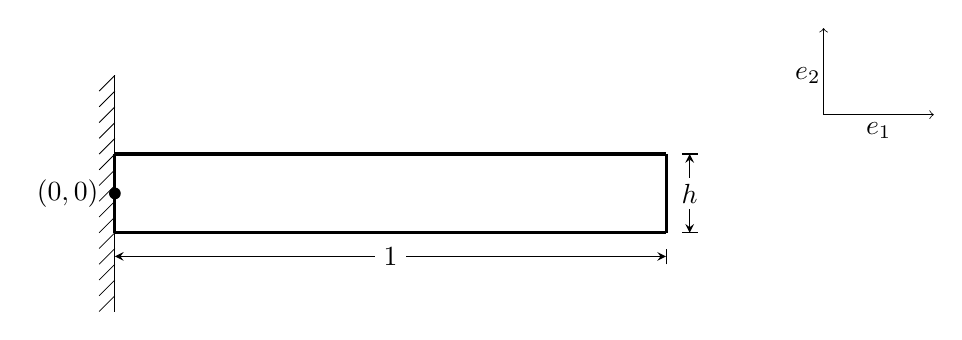
\begin{tikzpicture}
            
            \draw[line width = 0.4mm] (0,0.5) -- (7,0.5);
            \draw[line width = 0.4mm] (0,-0.5) -- (7,-0.5);
            \draw[line width = 0.4mm] (7,-0.5) -- (7,0.5);
            \draw[line width = 0.4mm] (0,-0.5) -- (0,0.5);
            
            \draw[line width = 0.1mm] (0,1.5) -- (0,-1.5);
            
            \draw[line width = 0.1mm] (0,1.5) -- (-0.2,1.3);
            \draw[line width = 0.1mm] (0,1.3) -- (-0.2,1.1);
            \draw[line width = 0.1mm] (0,1.1) -- (-0.2,0.9);
            \draw[line width = 0.1mm] (0,0.9) -- (-0.2,0.7);
            \draw[line width = 0.1mm] (0,0.7) -- (-0.2,0.5);
            \draw[line width = 0.1mm] (0,0.5) -- (-0.2,0.3);
            \draw[line width = 0.1mm] (0,0.3) -- (-0.2,0.1);
            \draw[line width = 0.1mm] (0,0.1) -- (-0.2,-0.1);
            \draw[line width = 0.1mm] (0,-0.1) -- (-0.2,-0.3);
            \draw[line width = 0.1mm] (0,-0.3) -- (-0.2,-0.5);
            \draw[line width = 0.1mm] (0,-0.5) -- (-0.2,-0.7);
            \draw[line width = 0.1mm] (0,-0.7) -- (-0.2,-0.9);
            \draw[line width = 0.1mm] (0,-0.9) -- (-0.2,-1.1);
            \draw[line width = 0.1mm] (0,-1.1) -- (-0.2,-1.3);
            \draw[line width = 0.1mm] (0,-1.3) -- (-0.2,-1.5);
            
            \node at (7.3,0) {$h$};
            \draw[-stealth] (7.3,0.2) -- (7.3,0.5);
            \draw (7.2,0.5) -- (7.4,0.5);
            \draw[-stealth] (7.3,-0.2) -- (7.3,-0.5);
            \draw (7.2,-0.5) -- (7.4,-0.5);
            
            \node at (3.5,-0.8) {$1$};
            \draw[stealth-] (0,-0.8) -- (3.3,-0.8);
            \draw[stealth-] (7,-0.8) -- (3.7,-0.8);
            \draw (7,-0.9) -- (7,-0.7);
            
            \draw[line width = 0.1mm,->] (9,1) -- (10.4,1);
            \draw[line width = 0.1mm,->] (9,1) -- (9,2.1);
            \node at (9.7,0.8) {$e_1$};
            \node at (8.8,1.5) {$e_2$};
            
            \node at (-0.6,0) {$(0,0)$};
            \node at (0,0)[circle,fill,inner sep=1.5pt]{};
            
        \end{tikzpicture}
        \caption{A cantilever two-dimensional elastic body.}
    \end{figure} 

    % Placeholder for boundary conditions of 2D cantilever
    Boundary Conditions:
    \begin{eqnarray*}
        u & = & 0 \quad \textrm{ where } x_1 = 0\\
        Tn & = & 0 \quad \textrm{ on the rest of the body }
    \end{eqnarray*} With $n$ the outward normal vector to $\Omega$.
\end{frame}

\begin{frame}{Three-dimensional cantilever elastic body}
    \begin{columns}[T] % align columns
        \begin{column}{.6\textwidth}
            \only<1->{ % Frame 1: Equations of motion
                Equations of motion
                \begin{eqnarray*}
                    \partial_t^2 u & = & \textrm{div}T + Q
                \end{eqnarray*}
                with
                \begin{eqnarray*}
                    \textrm{div}  T & = &
                    \begin{bmatrix}
                        \partial_1 \sigma_{11} + \partial_2 \sigma_{12} + \partial_3 \sigma_{13} \\
                        \partial_1 \sigma_{21} + \partial_2 \sigma_{22} + \partial_3 \sigma_{23} \\
                        \partial_1 \sigma_{31} + \partial_2 \sigma_{32} + \partial_3 \sigma_{33}
                    \end{bmatrix}.\label{eq:3D_Model:divT-D}
                \end{eqnarray*}
            }
            \only<1->{ % Frame 1: Constitutive equations
                Constitutive equations
                \begin{eqnarray*}
                    T = \frac{1}{\gamma(1+\nu)} \mathcal{E} + \frac{\nu}{\gamma(1+\nu)(1-2\nu)}\textrm{Tr}(\mathcal{E})I
                \end{eqnarray*}
            }
        \end{column}
        
        \begin{column}{.4\textwidth}
            \only<2->{ % Frame 2: Parameter descriptions
                \textbf{Description:}
                \begin{itemize}
                    \item[-] \( u \): Displacement vector in 3D
                    \item[-] \( T \): Stress tensor
                    \item[-] \( Q \): External distributed load in 3D
                    \item[-] \( \gamma \): Elasticity modulus
                    \item[-] \( \nu \): Poisson's ratio
                \end{itemize}
            }
        \end{column}
    \end{columns}
\end{frame}

\begin{frame}{Three-dimensional cantilever elastic body - Boundary Conditions}
    \begin{figure}[h!]
        \centering
        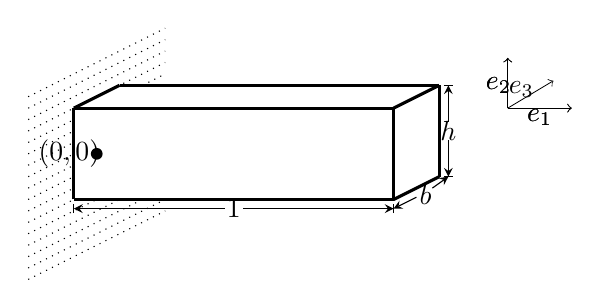
\begin{tikzpicture}[scale=0.58]
            
            \draw[line width = 0.4mm] (-0.5,1) -- (6.5,1);
            \draw[line width = 0.4mm] (-0.5,-1) -- (6.5,-1);
            \draw[line width = 0.4mm] (6.5,-1) -- (6.5,1);
            \draw[line width = 0.4mm] (-0.5,-1) -- (-0.5,1);
            
            \draw[line width = 0.4mm] (0.5,1.5) -- (7.5,1.5);
            \draw[line width = 0.4mm] (7.5,-0.5) -- (7.5,1.5);
            
            
            \draw[line width = 0.4mm] (-0.5,1) -- (0.5,1.5);
            \draw[line width = 0.4mm] (6.5,1) -- (7.5,1.5);
            \draw[line width = 0.4mm] (6.5,-1) -- (7.5,-0.5);
            
            
            
            \draw[scale=0.5, domain=-3:3, smooth, variable=\x,dotted] plot ({\x}, {0.5*\x+4});
            \draw[scale=0.5, domain=-3:3, smooth, variable=\x,dotted] plot ({\x}, {0.5*\x+3.5});
            \draw[scale=0.5, domain=-3:3, smooth, variable=\x,dotted] plot ({\x}, {0.5*\x+3});
            \draw[scale=0.5, domain=-3:3, smooth, variable=\x,dotted] plot ({\x}, {0.5*\x+2.5});
            
            \draw[scale=0.5, domain=-3:-1, smooth, variable=\x,dotted] plot ({\x}, {0.5*\x+2});
            \draw[scale=0.5, domain=2:3, smooth, variable=\x,dotted] plot ({\x}, {0.5*\x+2});
            
            \draw[scale=0.5, domain=-3:-1, smooth, variable=\x,dotted] plot ({\x}, {0.5*\x+1.5});
            \draw[scale=0.5, domain=-3:-1, smooth, variable=\x,dotted] plot ({\x}, {0.5*\x+1});
            \draw[scale=0.5, domain=-3:-1, smooth, variable=\x,dotted] plot ({\x}, {0.5*\x+0.5});
            \draw[scale=0.5, domain=-3:-1, smooth, variable=\x,dotted] plot ({\x}, {0.5*\x});
            \draw[scale=0.5, domain=-3:-1, smooth, variable=\x,dotted] plot ({\x}, {0.5*\x-0.5});
            \draw[scale=0.5, domain=-3:-1, smooth, variable=\x,dotted] plot ({\x}, {0.5*\x-1});
            \draw[scale=0.5, domain=-3:-1, smooth, variable=\x,dotted] plot ({\x}, {0.5*\x-1.5});
            \draw[scale=0.5, domain=-3:0, smooth, variable=\x,dotted] plot ({\x}, {0.5*\x-2});
            \draw[scale=0.5, domain=-3:1, smooth, variable=\x,dotted] plot ({\x}, {0.5*\x-2.5});
            \draw[scale=0.5, domain=-3:2, smooth, variable=\x,dotted] plot ({\x}, {0.5*\x-3});
            \draw[scale=0.5, domain=-3:3, smooth, variable=\x,dotted] plot ({\x}, {0.5*\x-3.5});
            \draw[scale=0.5, domain=-3:3, smooth, variable=\x,dotted] plot ({\x}, {0.5*\x-4});
            
            %\node at (6.9,1) {$b$};
            %\node at (6.65,0) {$h$};
            %\node at (3.2,-1.2) {$\ell = 1$};
            
            \draw[line width = 0.1mm,->] (9,1) -- (10,1.6);
            \draw[line width = 0.1mm,->] (9,1) -- (10.4,1);
            \draw[line width = 0.1mm,->] (9,1) -- (9,2.1);
            \node at (9.3,1.4) {$e_3$};
            \node at (9.7,0.8) {$e_1$};
            \node at (8.8,1.5) {$e_2$};
            
            \node at (7.7,0.5) {$h$};
            \draw[-stealth] (7.7,0.7) -- (7.7,1.5);
            \draw (7.6,1.5) -- (7.8,1.5);
            \draw[-stealth] (7.7,0.3) -- (7.7,-0.5);
            \draw (7.6,-0.5) -- (7.8,-0.5);
            
            \node at (3,-1.2) {$1$};
            \draw[stealth-] (-0.5,-1.2) -- (2.8,-1.2);
            \draw[stealth-] (6.5,-1.2) -- (3.2,-1.2);
            \draw (6.5,-1.3) -- (6.5,-1.1);
            \draw (-0.5,-1.3) -- (-0.5,-1.1);
            
            \node at (7.2,-0.9) {$b$};
            \draw[stealth-] (7.7,-0.5) -- (7.35,-0.75);
            \draw[stealth-] (6.5,-1.2) -- (7,-0.95);
            
            \draw[line width = 0.1mm,->] (9,1) -- (10.4,1);
            \draw[line width = 0.1mm,->] (9,1) -- (9,2.1);
            \node at (9.7,0.8) {$e_1$};
            \node at (8.8,1.5) {$e_2$};
            
            \node at (-0.6,0) {$(0,0)$};
            \node at (0,0)[circle,fill,inner sep=1.5pt]{};
            
            %\node at (-1.4,-1.3) {$(0,-\frac{h}{2},-\frac{b}{2})$};
            %\node at (-1.4,1) {$(0,\frac{h}{2},-\frac{b}{2})$};
            %\node at (0.5,1.8) {$(0,\frac{h}{2},\frac{b}{2})$};
            
            %\node at (6,-1.3) {$(1,-\frac{h}{2},-\frac{b}{2})$};
            %\node at (6.3,0.7) {$(1,\frac{h}{2},-\frac{b}{2})$};
            %\node at (7.5,1.8) {$(1,\frac{h}{2},\frac{b}{2})$};
            %\node at (8.4,-0.4) {$(1,-\frac{h}{2},\frac{b}{2})$};
            
        \end{tikzpicture}
        \caption{Cantilever Three-Dimensional Elastic Body with Rectangular Cross-Section.}
    \end{figure} 
    Boundary Conditions:
    \begin{eqnarray*}
        u & = & 0 \quad \textrm{ where } x_1 = 0\\
        Tn & = & 0 \quad \textrm{ on the rest of the body }
    \end{eqnarray*} With $n$ the outward normal vector to $\Omega$.
\end{frame}

\begin{frame}{Theory summary}
    
\end{frame}

\begin{frame}{Eigenvalue problem - Timoshenko model}
    Case $\boldsymbol{\lambda<\alpha}$

    Denote the roots of (\ref{TE7}) by $\pm \mu$ and $\pm \omega i$. Thus the general solution is given by
    \begin{eqnarray*}
    \begin{bmatrix}
    u(x)\\ \phi(x)
    \end{bmatrix}
    &=&
    A
    \begin{bmatrix}
    \sinh (\mu x) \\ \frac{\lambda+\mu^{2}}{\mu}\cosh (\mu x)
    \end{bmatrix}
    +
    B
    \begin{bmatrix}
    \cosh (\mu x) \\ \frac{\lambda+\mu^{2}}{\mu}\sinh (\mu x)
    \end{bmatrix}
    +
    C
    \begin{bmatrix}
    \sin (\omega x) \\ -\frac{\lambda-\omega^{2}}{\omega}\cos (\omega x)
    \end{bmatrix}\\
    &&
    +
    D
    \begin{bmatrix}
    \cos (\omega x) \\ \frac{\lambda-\omega^{2}}{\omega}\sin (\omega x)
    \end{bmatrix}.
    \end{eqnarray*}
\end{frame}

\begin{frame}{Eigenvalue problem - Timoshenko model}
    Case $\boldsymbol{ \lambda=\alpha}$

    In this case the roots of (\ref{TE7}) are $0$ with multiplicity 2, and $\pm \omega i$. The general solution is
    \begin{eqnarray*}
        \begin{bmatrix}
            u(x)\\ \phi(x)
        \end{bmatrix}
        =
        A
        \begin{bmatrix}
            0 \\1
        \end{bmatrix}
        +
        B
        \begin{bmatrix}
            1 \\ \alpha x
        \end{bmatrix}
        +
        C
        \begin{bmatrix}
            \sin (\omega x) \\ -\frac{\lambda-\omega^{2}}{\omega}\cos (\omega x)
        \end{bmatrix}
        +
        D
        \begin{bmatrix}
            \cos (\omega x) \\ \frac{\lambda-\omega^{2}}{\omega}\sin (\omega x)
        \end{bmatrix}.\label{T9}
    \end{eqnarray*}
\end{frame}

\begin{frame}{Eigenvalue problem - Timoshenko model}
    Case $\boldsymbol{\lambda>\alpha}$

    All the roots of (\ref{TE7}) are complex. Denote them by $\pm \theta i$ and $\pm \omega i$. The general solution is
    \begin{eqnarray*}
    \begin{bmatrix}
    u(x)\\ \phi(x)
    \end{bmatrix}
    &=&
    A
    \begin{bmatrix}
    \sin (\theta  x) \\-\frac{\lambda-\theta^{2}}{\theta}\cos (\theta x)
    \end{bmatrix}
    +
    B
    \begin{bmatrix}
    \cos (\theta x) \\ \frac{\lambda-\theta^{2}}{\theta}\sin (\theta x)
    \end{bmatrix}
    +
    C
    \begin{bmatrix}
    \sin (\omega x) \\ -\frac{\lambda-\omega^{2}}{\omega}\cos (\omega x)
    \end{bmatrix}\\
    &&
    +
    D
    \begin{bmatrix}
    \cos (\omega x) \\ \frac{\lambda-\omega^{2}}{\omega}\sin (\omega x)
    \end{bmatrix}.\label{T10}
    \end{eqnarray*}
\end{frame}

\begin{frame}{Eigenvalue problem - FEM}
    For the eigenvalue problem, assume that $M_{f}Q^I = 0$ so that 
\begin{eqnarray}
		M\ddot{\bar{u}} & = & K\bar{u}.\label{eq:2DFEM:M2}
\end{eqnarray}

$\bar{u} = \langle u, \partial_1 u, \partial_2 u, \partial_{12} u \rangle$


$\bar{u} = \langle u, \partial_1 u, \partial_2 u, \partial_3 u, \partial_{11} u, \partial_{12}u, \partial_{13}u,\partial_{22}u,\partial_{23}u, \partial_{33}u,$\\$ \partial_{111}u, \partial_{112}u, \partial_{113}u, \partial_{121}u, \partial_{122}u, \partial_{123}u, \partial_{133}u,\partial_{223}u,\partial_{233}u,\partial_{333}u \rangle$
\end{frame}

\begin{frame}{LVV09}
    
\end{frame}

\begin{frame}{Comparison of two and three-dimensional models}
    
\end{frame}

\end{document}
